\chapter{Messung, Dichtematrizen und Entropie}

Das Doppelspalt-Experiment enthält das Messproblem in seiner kleinsten brauchbaren Form. Solange zwei Alternativen kohärent bleiben, interferieren ihre Amplituden. Sobald ein anderes System eine Aufzeichnung darüber erhält, welche Alternative gewählt wurde, verschränken sich das Objekt und das aufzeichnende System, und die Interferenz verändert sich. Wir werden diesen Mechanismus präzisieren, bevor wir Spur, Dichtematrix und Entropie einführen---die Sprache, die wir brauchen, um Verschränkung quantitativ zu erfassen.

\section{Das Doppelspaltexperiment neu aufbauen}

Betrachten wir ein diskretes Modell mit einer Quelle am Ort \(0\), zwei Öffnungen \(A\) und \(B\) sowie einem Schirm, dessen mögliche Auftrefforte durch orthonormale Zustände \(\{|m\rangle\}\) dargestellt werden. Das Teilchen kann ein Elektron, ein Photon oder ein beliebiges anderes Quantenobjekt sein. Wir nennen es Elektron und vernachlässigen seinen Eigendrehimpuls, sodass hier nur der Ort als Freiheitsgrad betrachtet wird. Der übrige Teil der Barriere ist geschlossen: Ein Elektron, das einen anderen Ort als \(A\) oder \(B\) erreicht, wird reflektiert.

Das strukturelle Prinzip ist die Linearität. Wenn sich zwei Zustände gemäß
\begin{equation}
|A\rangle\longrightarrow |A'\rangle,
\qquad
|B\rangle\longrightarrow |B'\rangle,
\end{equation}
entwickeln, entwickelt sich jede Überlagerung mit denselben Koeffizienten:
\begin{equation}
\alpha|A\rangle+\beta|B\rangle
\longrightarrow
\alpha|A'\rangle+\beta|B'\rangle.
\end{equation}

Bei einer symmetrischen Anordnung speist die Quelle beide Öffnungen mit gleicher Amplitude. Wie an der Tafel lassen wir den gemeinsamen Normierungsfaktor weg:
\begin{equation}
|0\rangle\longrightarrow |A\rangle+|B\rangle.
\end{equation}
Der normierte Zustand wäre \((|A\rangle+|B\rangle)/\sqrt{2}\); der weggelassene Faktor spielt für das Interferenzargument keine Rolle.

Betrachten wir nun jeden Weg einzeln. Die Ausbreitung von den Öffnungen zum Schirm hat die Form
\begin{align}
|A\rangle &\longrightarrow \sum_m \psi_m|m\rangle, \\
|B\rangle &\longrightarrow \sum_m \phi_m|m\rangle.
\end{align}
Die komplexe Zahl \(\psi_m\) ist die Amplitude dafür, den Schirmort \(m\) zu erreichen, wenn der Ausgangsort \(A\) war; \(\phi_m\) ist die entsprechende Amplitude für den Ausgangsort \(B\).

\begin{figure}[htbp]
\centering
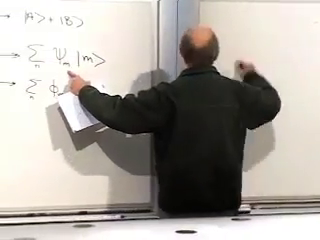
\includegraphics[width=0.68\textwidth]{lecture_07_figure_02.png}
\caption{Die getrennten Entwicklungen für den Weg durch \(A\) und den Weg durch \(B\) in der Schirmbasis.}
\lectureframe{00:05:39}
\end{figure}

Ist \(B\) geschlossen, beträgt die Wahrscheinlichkeit für den Schirmort \(m\)
\begin{equation}
P_A(m)=|\psi_m|^2.
\end{equation}
Ist \(A\) geschlossen,
\begin{equation}
P_B(m)=|\phi_m|^2.
\end{equation}
würde man nach klassischer Wahrscheinlichkeitsrechnung diese beiden Ergebnisse addieren, wenn beide Öffnungen offen sind. Die Quantenmechanik addiert stattdessen zunächst die Amplituden:
\begin{equation}
|A\rangle+|B\rangle
\longrightarrow
\sum_m(\psi_m+\phi_m)|m\rangle.
\end{equation}
An einem festen Schirmort gilt:
\begin{align}
P(m)
&=|\psi_m+\phi_m|^2 \\
&=|\psi_m|^2+|\phi_m|^2
  +\psi_m^*\phi_m+\phi_m^*\psi_m.
\end{align}

\begin{figure}[htbp]
\centering
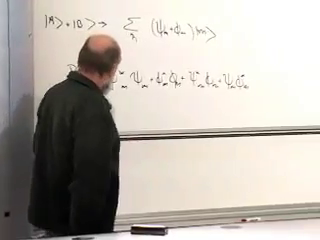
\includegraphics[width=0.70\textwidth]{lecture_07_figure_03.png}
\caption{Die Wahrscheinlichkeit am Schirm mit vier Termen. Die letzten beiden Terme sind die Interferenzterme.}
\lectureframe{00:09:21}
\end{figure}

An einem Symmetriepunkt gilt \(\psi_m=\phi_m\), und die beiden Alternativen verstärken einander. An einem Punkt, an dem sich ihre Phasen um \(\pi\) unterscheiden, gilt \(\psi_m=-\phi_m\), und die Wahrscheinlichkeit verschwindet. Jeder der beiden Wege allein kann zu diesem Punkt führen; sind jedoch beide Wege offen, kann dadurch verhindert werden, dass das Elektron dort ankommt. Damit stellt sich unausweichlich die Frage: Was ändert sich, wenn etwas aufzeichnet, durch welche Öffnung das Elektron gegangen ist?

\section{Der Detektor wird verschränkt}

Führen wir ein zusätzliches Zweizustandssystem mit den Zuständen \(|u\rangle\) und \(|d\rangle\) ein. In diesem Modell ist es nicht der Eigendrehimpuls des Elektrons, sondern ein minimales externes Messgerät. Anfangs ist der Detektor nicht ausgelöst:
\begin{equation}
|0,d\rangle.
\end{equation}
Die Wechselwirkung sei so eingerichtet, dass ein Durchgang durch \(A\) den Detektor umschaltet, während ein Durchgang durch \(B\) seinen Zustand unverändert lässt:
\begin{equation}
|0,d\rangle
\longrightarrow
|A,u\rangle+|B,d\rangle.
\end{equation}
Nachdem das Elektron die Öffnungen passiert hat, wechselwirkt es nicht mehr mit dem zusätzlichen Spin. Die beiden Zweige entwickeln sich daher wie folgt:
\begin{align}
|A,u\rangle &\longrightarrow \sum_m\psi_m|m,u\rangle, \\
|B,d\rangle &\longrightarrow \sum_m\phi_m|m,d\rangle,
\end{align}
Der Endzustand lautet somit
\begin{equation}
|\Psi\rangle
=\sum_m\left(\psi_m|m,u\rangle+\phi_m|m,d\rangle\right).
\end{equation}
Weg und Detektoraufzeichnung sind nun verschränkt. Am Detektor lässt sich ablesen, durch welche Öffnung das Elektron gegangen ist.

\begin{classroomqa}
\lecturetimestamp{00:13:24}
\audiencequestion{Ist die Wellenfunktion bereits kollabiert, wenn der Spin umschaltet?}
\lecturerresponse{Für das Elektron allein kann man von Kollaps sprechen: Die Wegalternativen interferieren nicht mehr. Im vollständigen System aus Elektron--und Detektor ist jedoch keiner der beiden Zweige verworfen worden. Der Zustand ist weiterhin \(|A,u\rangle+|B,d\rangle\). Bezieht man das Messgerät mit ein, wird aus der Aussage \emph{das Elektron ist kollabiert} die präzise Feststellung, dass eine Verschränkung zwischen System und--Messgerät entstanden ist.}
\end{classroomqa}

Der zusätzliche Spin ist lediglich ein praktischer Zeiger. Dieselbe Rolle kann jedes Paar unterscheidbarer Aufzeichnungen übernehmen: etwa ein ausgelöstes und ein nicht ausgelöstes Gerät oder ein emittiertes und ein nicht emittiertes Photon.

\begin{classroomqa}
\lecturetimestamp{00:15:17}
\audiencequestion{Hinterlässt der Durchgang durch die Metallplatte selbst immer eine Wegaufzeichnung?}
\lecturerresponse{Nicht unbedingt. Entscheidend ist, ob die Wechselwirkung die Platte in unterscheidbare Endzustände versetzt. Hat die Platte eine Anregungslücke und reicht die Energie des Elektrons nicht aus, sie anzuregen, muss keine bleibende innere Markierung entstehen. Eine bloße Wechselwirkung genügt nicht; die beiden Alternativen müssen mit unterscheidbaren Aufzeichnungen korreliert werden.}
\end{classroomqa}

\begin{classroomqa}
\lecturetimestamp{00:16:29}
\audiencequestion{Könnte der Rückstoß der Platte erkennen lassen, ob das Elektron durch die obere oder die untere Öffnung gegangen ist?}
\lecturerresponse{Nur wenn die entgegengesetzten Impulsüberträge Zustände der Platte erzeugen, die hinreichend gut unterscheidbar sind. Eine gut lokalisierte Platte besitzt bereits eine breite Impulswellenfunktion. Kleine Verschiebungen nach oben und unten können sich nahezu vollständig überlappen, sodass die Rückstoßzustände nicht orthogonal sind und keine eindeutige Wegaufzeichnung liefern. Hier schützt die Unschärferelation die Interferenz.}
\end{classroomqa}

Eine teilweise Aufzeichnung ist möglich. Wird der Detektor nur leicht angestoßen, müssen die beiden Aufzeichnungszustände nicht orthogonal sein. Dann wird die Interferenz abgeschwächt, aber nicht vollständig beseitigt. Für die formale Rechnung betrachten wir zunächst den Grenzfall einer vollständigen Messung:
\begin{equation}
\langle u|d\rangle=0.
\end{equation}

\section{Die Rechnung mit dem Projektor}

Berechnen wir nun die Wahrscheinlichkeit, dass das Elektron an einem festen Schirmort \(m\) ankommt, ohne nach dem Detektorergebnis zu fragen. Im zusammengesetzten Hilbertraum ist die Eigenschaft \emph{Elektron am Ort \(m\)} ein zweidimensionaler Unterraum, aufgespannt von
\begin{equation}
|m,u\rangle,\qquad |m,d\rangle.
\end{equation}
Der zugehörige Projektor lautet
\begin{equation}
\Pi_m
=|m,u\rangle\langle m,u|
 +|m,d\rangle\langle m,d|.
\end{equation}

\begin{figure}[htbp]
\centering
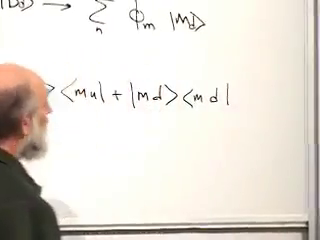
\includegraphics[width=0.66\textwidth]{lecture_07_figure_04.png}
\caption{Der Projektor auf eine feste Schirmposition, summiert über die beiden orthogonalen Detektoraufzeichnungen.}
\lectureframe{00:22:04}
\end{figure}

Das Wahrscheinlichkeitspostulat liefert
\begin{equation}
P(m)=\langle\Psi|\Pi_m|\Psi\rangle.
\end{equation}
Schreiben wir die Summen aus:
\begin{align}
P(m)
&=
\sum_{n,n'}
\left(\psi_n^*\langle n,u|+\phi_n^*\langle n,d|\right)
\notag\\
&\quad\times\Pi_m
\notag\\
&\quad\times
\left(\psi_{n'}|n',u\rangle+\phi_{n'}|n',d\rangle\right).
\end{align}
Die Orts-Skalarprodukte erzwingen \(n=m=n'\). Welche Terme übrig bleiben, hängt dann von den Skalarprodukten der Detektorzustände ab:
\begin{align}
\langle u|u\rangle&=1,
&
\langle d|d\rangle&=1,
&
\langle u|d\rangle&=\langle d|u\rangle=0.
\end{align}
Folglich gilt
\begin{equation}
P(m)=|\psi_m|^2+|\phi_m|^2.
\end{equation}

Die Kreuzterme wurden nicht einfach per Beschluss gestrichen. Sie verschwinden, weil die beiden Wegamplituden nun mit orthogonalen Vektoren im erweiterten Zustandsraum multipliziert werden. Damit Alternativen interferieren können, müssen sie nicht nur am Schirm denselben Endpunkt haben, sondern auch in jedem Freiheitsgrad übereinstimmen, der eine Aufzeichnung trägt.

\section{Was gilt als Messung?}

Das einfache Spinmodell liefert eine allgemeine Regel: Eine Messung findet statt, wenn eine Wechselwirkung eine Korrelation zwischen den Alternativen des Systems und unterscheidbaren Zuständen eines Messgeräts herstellt. Die folgenden Varianten prüfen diese Regel.

\begin{classroomqa}
\lecturetimestamp{00:26:53}
\audiencequestion{Was geschieht, wenn der Spin symmetrisch angeordnet ist und bei einem Durchgang durch eine der beiden Öffnungen umschaltet?}
\lecturerresponse{Dann tragen beide Zweige dieselbe Aufzeichnung, \(|A,u\rangle+|B,u\rangle=(|A\rangle+|B\rangle)\otimes|u\rangle\). Der Detektorzustand separiert sich ab und verrät nichts über den Weg; das Interferenzmuster bleibt daher erhalten.}
\end{classroomqa}

\begin{figure}[htbp]
\centering
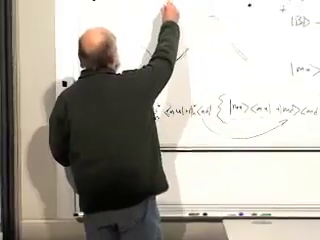
\includegraphics[width=0.68\textwidth]{lecture_07_figure_05.png}
\caption{Die Variante an der Tafel mit einem symmetrisch angeordneten Detektor, der auf beide Wege gleich reagiert.}
\lectureframe{00:27:14}
\end{figure}

\begin{figure}[htbp]
\centering
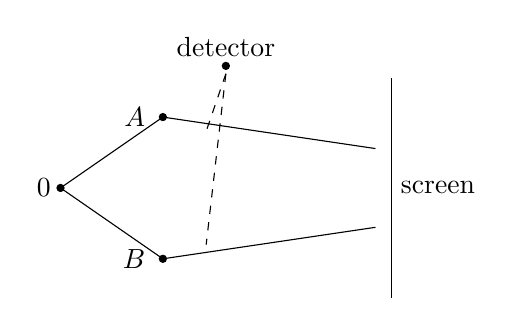
\begin{tikzpicture}[scale=1.0]
\fill (-2,0) circle (1.5pt);
\node[left] at (-2,0) {$0$};
\fill (-0.7,0.9) circle (1.5pt);
\node[left] at (-0.8,0.9) {$A$};
\fill (-0.7,-0.9) circle (1.5pt);
\node[left] at (-0.8,-0.9) {$B$};
\draw (-2,0) -- (-0.7,0.9);
\draw (-2,0) -- (-0.7,-0.9);
\draw (-0.7,0.9) -- (2.0,0.5);
\draw (-0.7,-0.9) -- (2.0,-0.5);
\draw (2.2,-1.4) -- (2.2,1.4);
\node[right] at (2.2,0) {screen};
\fill (0.1,1.55) circle (1.5pt);
\node[above] at (0.1,1.55) {detector};
\draw[dashed] (0.1,1.45) -- (-0.15,0.72);
\draw[dashed] (0.1,1.45) -- (-0.15,-0.72);
\end{tikzpicture}
\caption{Eine klare Rekonstruktion der symmetrischen Detektoranordnung: Beide Wege führen zum selben Detektorzustand.}
\end{figure}

\begin{classroomqa}
\lecturetimestamp{00:27:55}
\audiencequestion{Muss jemand den zusätzlichen Spin tatsächlich ablesen, bevor die Interferenz verschwindet?}
\lecturerresponse{Nein. Das Elektron hat seinen Weg bereits mit dem Spin korreliert. Man kann den Detektor zurücksetzen, das Experiment mit einzelnen Elektronen wiederholen und nur die Verteilung der Treffer am Schirm untersuchen. Die Interferenzstreifen fehlen auch dann, wenn niemand den Spin abliest; entscheidend ist die physikalische Aufzeichnung, nicht das menschliche Bewusstsein davon.}
\end{classroomqa}

\begin{classroomqa}
\lecturetimestamp{00:29:36}
\audiencequestion{Würde eine hinreichend leichte Platte, die zurückstößt, die Interferenz zerstören?}
\lecturerresponse{Ja, wenn der Rückstoß die Platte für die beiden Wege in orthogonale Impulszustände versetzt. Überlappen sich die verschobenen Wellenpakete weiterhin, wird die Interferenz nur teilweise zerstört. Die Masse allein ist nicht entscheidend, sondern die Unterscheidbarkeit der Endzustände der Platte.}
\end{classroomqa}

Strahlung ist ein weiterer, unvollkommener Aufzeichner. Ein beschleunigtes geladenes Teilchen kann ein Photon emittieren. Die nahe \(A\) emittierte Strahlung muss nicht denselben Zustand haben wie die nahe \(B\) emittierte; das elektromagnetische Feld kann daher Weg-Information bewahren. Bei einem langsam abgelenkten Elektron kann die Emissionswahrscheinlichkeit klein sein; in der Vorlesung wird zur Veranschaulichung ein Ereignis pro hundert Fälle geschätzt. Bei stärkerer Beschleunigung wird Strahlung und damit ein Verlust an Kontrast wahrscheinlicher. Entscheidend ist die qualitative Aussage: Auch ein unbeobachtetes Photon kann Kohärenz davontragen.

\begin{classroomqa}
\lecturetimestamp{00:32:00}
\audiencequestion{Wie lässt sich in einem realen Experiment mit unvollständigem Kontrast die Interferenzwahrscheinlichkeit bestimmen?}
\lecturerresponse{Man wiederholt das Experiment viele Male und schätzt aus den relativen Häufigkeiten die Verteilung am Schirm. Bei endlichen Stichproben und durch Aufzeichnungen in der Umgebung bleiben in nominell dunklen Bereichen Resttreffer. Die geschätzte Wahrscheinlichkeitsverteilung wird mit zunehmender Zahl der Durchläufe genauer, während Dekohärenzprozesse den physikalischen Kontrast der Interferenzstreifen verringern.}
\end{classroomqa}

\begin{classroomqa}
\lecturetimestamp{00:33:13}
\audiencequestion{Zerstört schon die Möglichkeit, den Weg zu bestimmen, die gesamte Interferenz?}
\lecturerresponse{Vollständige Unterscheidbarkeit zerstört sie vollständig. Teilweise Information führt zu einem teilweisen Verlust. Ein Detektor, der sich nur geringfügig dreht, hinterlässt zwei nicht orthogonale Aufzeichnungszustände. Liest man den Detektor ab, wird dadurch ein Weg wahrscheinlicher als der andere, aber nicht sicher; entsprechend werden die Interferenzstreifen verwischt, statt ausgelöscht.}
\end{classroomqa}

Seien \(|E_A\rangle\) und \(|E_B\rangle\) beliebige Aufzeichnungszustände. Der Gesamtzustand am Schirm lässt sich schreiben als
\begin{equation}
|\Psi\rangle
=\sum_m\left(
\psi_m|m\rangle|E_A\rangle
+\phi_m|m\rangle|E_B\rangle
\right).
\end{equation}
Lässt man das Aufzeichnungssystem unberücksichtigt, ergibt sich
\begin{align}
P(m)
&=|\psi_m|^2+|\phi_m|^2 \\
&\quad
+\psi_m^*\phi_m\langle E_A|E_B\rangle
+\phi_m^*\psi_m\langle E_B|E_A\rangle.
\end{align}
Die Überlappung \(\langle E_A|E_B\rangle\) ist somit der Kohärenzfaktor. Identische Aufzeichnungen erhalten die Interferenz vollständig; orthogonale Aufzeichnungen beseitigen sie; bei einer dazwischenliegenden Überlappung ist auch die Sichtbarkeit entsprechend dazwischenliegend.

\begin{classroomqa}
\lecturetimestamp{00:34:12}
\audiencequestion{Was geschieht, wenn nur gelegentlich Photonen emittiert werden und man ausschließlich die Ereignisse mit Photonemission betrachtet?}
\lecturerresponse{Diese ausgewählte Teilmenge zeigt im Allgemeinen eine schwächere Interferenz, weil ein Photon Weg-Information trägt. Der Verlust muss nicht vollständig sein: Die an den beiden Öffnungen emittierten Photonenwellenpakete können sich selbst überlappen, sodass auch die Strahlungsaufzeichnungen nicht perfekt orthogonal sein müssen.}
\end{classroomqa}

Der Beschuss durch die Umgebung verstärkt diesen Mechanismus. Luftmoleküle, Umgebungsphotonen und Materie in der Umgebung zeichnen fortwährend makroskopische Positionen auf. Ein Mensch oder der Mond bleibt nicht sichtbar in einer kohärenten Ortsüberlagerung: Masse verlangsamt die freie Ausbreitung, und die kontinuierliche Verschränkung mit der Umgebung unterdrückt beobachtbare Interferenz zwischen makroskopisch weit auseinanderliegenden Alternativen.

\begin{classroomqa}
\lecturetimestamp{00:36:02}
\audiencequestion{Ist das bereits eine Messtheorie und nicht bloß eine weitere Verwendung des Ausdrucks \emph{Kollaps des Wellenpakets}?}
\lecturerresponse{Dies ist der Mechanismus in einem bewusst exakt gewählten Beispiel. In einer Beschreibung, die nur das Elektron umfasst, bedeutet Kollaps, die außerdiagonalen Terme \(\psi^*\phi\) zu verwerfen. In der Beschreibung des zusammengesetzten Systems ist keine willkürliche Streichung nötig: Durch die Verschränkung mit orthogonalen Zuständen des Messgeräts stehen diese Terme für Messungen am Elektron allein nicht zur Verfügung. Komplexere Beispiele sollte man auf diese Struktur zurückführen.}
\end{classroomqa}

\begin{classroomqa}
\lecturetimestamp{00:38:04}
\audiencequestion{Ändert ein Gravitationsfeld, das den Weg krümmt, auf natürliche Weise das Strahlungsargument oder die Interferenzregel?}
\lecturerresponse{Die Einzelheiten der Strahlung können sich ändern, und die Quantenmechanik weist vor einer Wegmessung keine einzelne scharf bestimmte Bahn zu. An der allgemeinen Schlussfolgerung ändert sich nichts: Interferenz wird nur durch einen Freiheitsgrad unterdrückt, der unterscheidbare Weg-Information bewahrt. Für eine genauere Antwort muss zunächst ein konkreter Versuchsaufbau angegeben werden.}
\end{classroomqa}

\begin{classroomqa}
\lecturetimestamp{00:39:44}
\audiencequestion{Unterscheidet sich diese Interferenz von der Interferenz klassischer elektromagnetischer Wellen?}
\lecturerresponse{Bei vielen Photonen stimmt das beobachtete Muster mit der gewöhnlichen Welleninterferenz des elektromagnetischen Feldes überein. Das Einzelteilchenexperiment zeigt die tiefere quantenmechanische Aussage: Photonen und Elektronen treffen als einzelne Ereignisse ein, während ihre Quantenamplituden interferieren. Bei Elektronen ist die relevante Welle die Elektronenwellenfunktion, keine elektromagnetische Welle.}
\end{classroomqa}

\begin{classroomqa}
\lecturetimestamp{00:40:45}
\audiencequestion{Was geschieht mit den Anteilen der einfallenden Welle, die auf Bereiche zwischen \(A\) und \(B\) gerichtet sind?}
\lecturerresponse{In diesem bewusst diskreten Modell ist der übrige Teil der Barriere versperrt. Diese Anteile werden reflektiert und tragen nicht zur transmittierten Amplitude am Schirm bei. Das Modell isoliert die beiden transmittierten Alternativen, ohne zu behaupten, dass ein realer Strahl nur zwei Impulskomponenten hat.}
\end{classroomqa}

\section{Die Katze, der Schirm und die verschiebbare Schnittstelle}

Dieselbe Mathematik gilt für Schrödingers Katze Schr\"odinger. Die Zustände der Waffe seien \(|U\rangle\) und \(|F\rangle\) für nicht abgefeuert und abgefeuert, die Zustände der Katze \(|L\rangle\) und \(|D\rangle\) für lebendig und tot. Ausgehend von einer lebendigen Katze und einer nicht abgefeuerten Waffe kann die Wechselwirkung zu folgendem Zustand führen:
\begin{equation}
|\Psi_{\mathrm{cat}}\rangle
=\alpha|L,U\rangle+\beta|D,F\rangle.
\end{equation}
Die Katze allein befindet sich nicht im kohärenten Zustand \(\alpha|L\rangle+\beta|D\rangle\). Sie ist mit einer Waffe verschränkt, die die Alternative aufgezeichnet hat. Ein Blick auf die Waffe kann den Zweig der Katze offenbaren, und die orthogonalen Aufzeichnungen der Waffe beseitigen gewöhnliche Interferenz zwischen lebend--und tot im Katzensystem.

\begin{classroomqa}
\lecturetimestamp{00:41:18}
\audiencequestion{Befindet sich die Katze selbst in einer Überlagerung aus lebendig und tot?}
\lecturerresponse{Nicht im einfachen, isolierten Sinn. Das zusammengesetzte System aus Katze--und Waffe befindet sich in einer Überlagerung korrelierter Alternativen: lebendig und Waffe nicht abgefeuert sowie tot und Waffe abgefeuert. Das Katzensystem ist mit einer Waffe verschränkt, die eine Aufzeichnung trägt, genau wie der Elektronenweg mit dem zusätzlichen Spin verschränkt ist.}
\end{classroomqa}

Auch der abschließende Schirm muss als Messgerät behandelt werden. Ein Elektron, das bei \(m\) ankommt, kann ein fotografisches Korn schwärzen, einen Szintillator ein Photon aussenden lassen oder eines von mehreren lokal angeordneten Zweizustandsgeräten umschalten. Die Markierung wird mit dem Auftreffort korreliert.

\begin{classroomqa}
\lecturetimestamp{00:43:38}
\audiencequestion{Warum dürfen wir von Wahrscheinlichkeiten am abschließenden Schirm sprechen, statt für immer nur Zustandsvektoren weiterzuentwickeln?}
\lecturerresponse{Das Wahrscheinlichkeitspostulat ordnet der Eigenschaft \emph{Ankunft bei \(m\)} den Wert \(\langle\Pi_m\rangle\) zu. Im vollständigen physikalischen Experiment hinterlässt der Schirm anschließend eine Ortsaufzeichnung. Der Projektor liefert die Wahrscheinlichkeit; Schwärzung, Szintillation oder das Umschalten eines lokalen Detektors realisieren die Messung, deren Statistik erfasst wird.}
\end{classroomqa}

\begin{classroomqa}
\lecturetimestamp{00:45:00}
\audiencequestion{Warum sprechen wir von einer Messung am Schirm, aber nicht von einer Wahrscheinlichkeit für den Durchgang durch \(A\) oder \(B\)?}
\lecturerresponse{Wegwahrscheinlichkeiten lassen sich nur dann zuordnen und überprüfen, wenn ein Wegaufzeichner installiert ist. Ohne eine solche Aufzeichnung bleiben die Alternativen kohärent und müssen als Amplituden addiert werden. Am Schirm wird ein ortsempfindliches Messgerät vorausgesetzt. Der Unterschied liegt nicht in einem bevorzugten Zeitpunkt, sondern darin, ob eine entsprechende Messwechselwirkung eingerichtet wurde.}
\end{classroomqa}

Die Grenze zwischen System und Messgerät lässt sich verschieben. Bezieht man einen Beobachter mit Aufzeichnungszuständen \(|O_u\rangle\) und \(|O_d\rangle\) ein, gilt:
\begin{equation}
|A,u\rangle+|B,d\rangle
\longrightarrow
|A,u,O_u\rangle+|B,d,O_d\rangle.
\end{equation}
Ein weiterer Beobachter kann seinerseits mit dem ersten korreliert werden. Der Rauch in der Katzenbox, die Waffe, die Katze, Schr\"odinger und Wigner können alle in eine längere Verschränkungskette einbezogen werden. Wo immer man die Schnittstelle zieht, müssen die Korrelationen konsistent bleiben: Fragt Wigner später Schr\"odinger, was er gesehen hat, stimmen ihre Aufzeichnungen überein.

\begin{classroomqa}
\lecturetimestamp{00:47:24}
\audiencequestion{Wo genau endet das System und wo beginnt der messende Beobachter?}
\lecturerresponse{Die Quantenmechanik legt keine eindeutige, zweckmäßige Schnittstelle fest. Man kann die Beschreibung des Elektrons allein kollabieren lassen, den Detektor einbeziehen und eine größere Beschreibung kollabieren lassen oder einen Beobachter einbeziehen und den verschränkten Zustand nochmals erweitern. Physikalisch erforderlich ist die Konsistenz aller zugänglichen Wahrscheinlichkeiten und Aufzeichnungen, nicht eine eindeutige Grenze der Beschreibung.}
\end{classroomqa}

\begin{classroomqa}
\lecturetimestamp{00:49:47}
\audiencequestion{Kommt die Unschärferelation ins Spiel, weil die Wegmessung den Vorgang stört?}
\lecturerresponse{Ja. Das Rückstoßbeispiel macht den Zusammenhang deutlich: Die Lokalisierung der Platte führt zu einer Impulsunschärfe, durch die kleine wegabhängige Impulsüberträge möglicherweise nicht unterscheidbar werden. Allgemeiner gilt: Eine quantenmechanische Messung ist erst abgeschlossen, wenn die Verschränkung zwischen System und--Messgerät den Zustand verändert hat; diese Änderung kann spätere Interferenz beeinflussen.}
\end{classroomqa}

Das unterscheidet die Situation deutlich vom klassischen Ideal. Klassisch stellt man sich vor, eine Messung beliebig schonend durchführen und Informationen mit vernachlässigbarer Störung gewinnen zu können. Hier erfordert die Gewinnung von Weg-Information eine Korrelation mit einem Messgerät. Das verändert den Gesamtzustand tatsächlich und damit auch das Ergebnis eines späteren Interferenzexperiments.

\begin{classroomqa}
\lecturetimestamp{00:52:06}
\audiencequestion{Was geschieht, wenn der Abstand zwischen \(A\) und \(B\) sehr groß wird?}
\lecturerresponse{Dafür gibt es keine allgemeingültige neue Regel. In dieser Anordnung aus Quelle und Barriere können die Amplituden, sehr weit entfernte Öffnungen zu erreichen, schlicht klein werden, sodass die meisten Teilchen auf den versperrten Bereich treffen. Abgesehen von solchen vom Versuchsaufbau abhängigen Änderungen von \(\psi_m\) und \(\phi_m\) entscheidet der Abstand allein nicht darüber, ob die Kohärenz erhalten bleibt.}
\end{classroomqa}

\begin{classroomqa}
\lecturetimestamp{00:53:04}
\audiencequestion{Ist die Linearität der Quantenentwicklung fundamental exakt, und warum gilt sie in der Natur?}
\lecturerresponse{Linearität ist eine empirische Grundlage der Quantenmechanik. Kleine nichtlineare Abweichungen lassen sich bekanntermaßen nur schwer logisch widerspruchsfrei formulieren und beeinträchtigen tendenziell die Struktur. Warum physikalische Aussagen der Logik von Unterräumen statt der klassischen Mengenlogik folgen, wird hier nicht erklärt; die Vorlesung behandelt es als Tatsache der Natur.}
\end{classroomqa}

\begin{classroomqa}
\lecturetimestamp{00:54:53}
\audiencequestion{Kann eine spätere Beobachtung den früheren Weg offenbaren und dadurch verändern, ob Interferenz stattgefunden hat?}
\lecturerresponse{Kann eine spätere Beobachtung den Weg offenbaren, muss ein physikalischer Freiheitsgrad eine wegabhängige Aufzeichnung bewahrt haben. Diese Aufzeichnung beeinflusst die Kohärenz bereits; niemand muss sie ablesen. Die Kausalität muss weiterhin gewahrt bleiben, und eine abstrakte Behauptung zur verzögerten Wahl lässt sich ohne Angabe des vollständigen raumzeitlichen Aufbaus und des Messgeräts nicht beurteilen.}
\end{classroomqa}

\begin{classroomqa}
\lecturetimestamp{00:56:47}
\audiencequestion{Was geschieht, wenn unmittelbar hinter den Öffnungen eine Blasenkammer aufgestellt wird?}
\lecturerresponse{Eine Spur, die die beiden austretenden Wege unterscheidet, ist eine eindeutige Markierung und zerstört daher ihre Interferenz. Dafür reicht eine dünne Schicht, die den Weg aufzeichnet. Bewahrt ein nachgeschaltetes Gerät nicht genügend Information, um auf die zuvor benutzte Öffnung zu schließen, ist es nicht automatisch ein Welche-Weg-Detektor.}
\end{classroomqa}

\begin{classroomqa}
\lecturetimestamp{00:59:29}
\audiencequestion{Wenn die Welt bereits stark verschränkt ist, wie kann ein Interferenzexperiment dann jemals mit unverschränkten Systemen beginnen?}
\lecturerresponse{Bei der Präparation müssen die relevanten Freiheitsgrade hinreichend isoliert, zurückgesetzt oder konditioniert werden, sodass die Alternativen anfangs dieselbe Aufzeichnung in der Umgebung haben. Eine frühere Spur in einer Blasenkammer kann nicht einfach ignoriert werden, wenn sie weiterhin mit dem Weg korreliert ist. Interferenz erfordert anfangs eine annähernd Produktform zwischen dem kontrollierten System und dem relevanten Aufzeichner.}
\end{classroomqa}

\begin{classroomqa}
\lecturetimestamp{01:01:04}
\audiencequestion{Wie lässt sich nach einer Messung praktisch eine Entschränkung erreichen?}
\lecturerresponse{Man konditioniert auf ein eindeutig beobachtetes Ergebnis. Wird der Spin als nach oben gerichtet gemessen, behält der Beobachter den Zweig \(|A,u\rangle\) bei und verwirft die Alternative aus der Arbeitsbeschreibung. Dieser bedingte Produktzustand kann als neuer Ausgangspunkt dienen. Der vollständige Zustand einschließlich Beobachter kann weiterhin verschränkt sein; relativ zum aufgezeichneten Ergebnis ist die ausgewählte Präparation jedoch eindeutig.}
\end{classroomqa}

Diese verschachtelte Hierarchie löst nicht jede Deutungsfrage, macht aber die operationale Konsistenz sichtbar. System, Detektor, Beobachter und Beobachter des Beobachters können alle einbezogen werden. Wo immer man die Beschreibung schneidet: Richtig korrelierte Aufzeichnungen widersprechen einander später nicht.

\section{Von der Verschränkung zur Entropie}

Die Diskussion über Messungen ist weiter gegangen als geplant, hat aber die nächste Frage aufgeworfen: Wie lässt sich der Grad der Verschränkung messen? Zwei Spins im Produktzustand
\begin{equation}
|u\rangle\otimes|u\rangle
\end{equation}
sind nicht verschränkt. Jedes Teilsystem hat seinen eigenen eindeutigen Zustand, und die Beobachtung des einen liefert keine neue Information über das andere. Verschränkte Zustände lassen sich nicht auf diese Weise faktorisieren. Ein gängiges quantitatives Maß ist die Verschränkungsentropie; dafür benötigen wir jedoch zunächst den gewöhnlichen Entropiebegriff und anschließend seine quantenmechanische Form.

\section{Klassische Entropie als fehlende Information}

Beginnen wir mit einem klassischen System, das eine endliche Menge von \(N\) möglichen Zuständen hat. Die Entropie ist hier eine Eigenschaft des Systems zusammen mit unserem Wissen darüber. Angenommen, wir wissen nur, dass sich das System in einem von \(n\) gleichwahrscheinlichen Zuständen befindet. Dann gilt
\begin{equation}
S=\log n.
\end{equation}
Ist \(n=1\), ist der Zustand bekannt und \(S=0\). Ist \(n=N\), weiß man über den Zustandsraum selbst hinaus nichts, und die Entropie ist maximal: \(S_{\max}=\log N\).

Der Logarithmus zählt unabhängige Ja--Nein-Entscheidungen additiv. Für \(M\) klassische Spins gibt es \(2^M\) Konfigurationen, also
\begin{equation}
\log(2^M)=M\log 2.
\end{equation}
Bis auf die Wahl der Logarithmenbasis zählt die Entropie somit die Menge an binärer Information, die in der Beschreibung fehlt.

Für eine allgemeine Wahrscheinlichkeitsverteilung \(p_i\) lautet die passende Definition
\begin{equation}
S=-\sum_i p_i\log p_i.
\end{equation}

\begin{classroomqa}
\lecturetimestamp{01:14:17}
\audiencequestion{Warum steht in der Entropieformel ein Minuszeichen?}
\lecturerresponse{Jede von null verschiedene Wahrscheinlichkeit erfüllt \(0<p_i\leq 1\), also gilt \(\log p_i\leq 0\). Durch das Minuszeichen ist die Entropie nichtnegativ. Für \(p_i=0\) wird der Beitrag durch den Grenzwert \(p_i\log p_i\to0\) definiert.}
\end{classroomqa}

Für die Gleichverteilung
\begin{equation}
p_i=
\begin{cases}
1/n, & i\in\mathcal N,\\
0, & i\notin\mathcal N,
\end{cases}
\qquad |\mathcal N|=n,
\end{equation}
wird die allgemeine Formel zu
\begin{align}
S
&=-n\left(\frac1n\right)\log\left(\frac1n\right)\\
&=\log n.
\end{align}
Damit ergibt sich wieder die elementare Zähldefinition. Für eine Verteilung, die mit Sicherheit auf einen einzigen Zustand konzentriert ist, gilt \(S=0\).

\begin{figure}[htbp]
\centering
\includegraphics[width=0.66\textwidth]{lecture_07_figure_07.png}
\caption{Die Tafel fasst \(S=\log n\), die Shannon-Formel und die Überprüfung für gleiche Wahrscheinlichkeiten zusammen.}
\lectureframe{01:16:08}
\end{figure}

\begin{classroomqa}
\lecturetimestamp{01:17:35}
\audiencequestion{Wie groß ist die maximale Entropie eines Systems mit \(N\) Zuständen, und was ist in diesem Fall bekannt?}
\lecturerresponse{Das Maximum beträgt \(\log N\) und wird von der Gleichverteilung \(p_i=1/N\) erreicht. Man weiß weiterhin, um welches System es sich handelt, und kennt damit seinen Zustandsraum; unbekannt ist, welchen dieser \(N\) Zustände es einnimmt.}
\end{classroomqa}

Die Differenz
\begin{equation}
I=S_{\max}-S
\end{equation}
ist die in diesem Zählsinn verfügbare Information. Entropie und Information sind zwei Seiten derselben Bilanz: Die Entropie erfasst jene Information, mit der sich der Zustand unterscheiden ließe, die uns aber nicht zur Verfügung steht.

\section{Die Spur: der quantenmechanische Ersatz für eine Summe}

Für einen Operator \(M\) und eine beliebige vollständige Orthonormalbasis \(\{|i\rangle\}\) definieren wir
\begin{equation}
\operatorname{Tr}M
=\sum_i\langle i|M|i\rangle.
\end{equation}

\begin{figure}[htbp]
\centering
\includegraphics[width=0.68\textwidth]{lecture_07_figure_08.png}
\caption{Die Spur als Summe der Diagonalelemente der Matrix.}
\lectureframe{01:21:20}
\end{figure}

Obwohl die Definition mithilfe einer Basis formuliert ist, ist das Ergebnis basisunabhängig. Für einen hermiteschen Operator kann man eine Eigenbasis wählen; dann gilt
\begin{equation}
\operatorname{Tr}M=\sum_i\lambda_i.
\end{equation}
Die Eigenwerte und damit auch ihre Summe hängen nicht von den Koordinaten ab, mit denen der Operator dargestellt wird.

\begin{classroomqa}
\lecturetimestamp{01:23:04}
\audiencequestion{Bedeutet die Diagonalform einer Matrix, dass sie invertierbar ist?}
\lecturerresponse{Nein. In der Diagonalform sind die Eigenwerte zu sehen; die Invertierbarkeit ist eine davon unabhängige Bedingung. Eine Diagonalmatrix ist genau dann invertierbar, wenn keiner ihrer diagonalen Eigenwerte null ist. Hermitesche Matrizen sind auch dann diagonalisierbar, wenn einige Eigenwerte verschwinden.}
\end{classroomqa}

Nach der Pause kehren wir kurz zur klassischen Wahrscheinlichkeit zurück. Eine klassische Observable ist eine Funktion \(f_i\) der Konfiguration, und ihr Mittelwert ist
\begin{equation}
\langle f\rangle_{\mathrm{cl}}=\sum_i p_i f_i.
\end{equation}
In den quantenmechanischen Formeln tritt die Spur an die Stelle der Summe über die Alternativen, ein Operator an die Stelle der klassischen Funktion und eine Dichtematrix an die Stelle der Wahrscheinlichkeitsverteilung.

\section{Statistische Gemische und die Dichtematrix}

Angenommen, jemand präpariert ein System in einem Zustand einer Orthonormalbasis, verrät uns aber nicht, welcher Zustand gewählt wurde. Es werden lediglich Präparationswahrscheinlichkeiten angegeben---zum Beispiel wird ein Spin mit Wahrscheinlichkeit \(3/4\) nach oben und mit Wahrscheinlichkeit \(1/4\) nach unten präpariert. Dies ist nicht die kohärente Superposition
\begin{equation}
\sqrt{\frac34}|u\rangle+\sqrt{\frac14}|d\rangle,
\end{equation}
denn es wurde keine relative Phase präpariert. Es handelt sich um ein statistisches Gemisch wohldefinierter Zustände. Quantenmechanische Wahrscheinlichkeiten bleiben auch dann bestehen, wenn ein reiner Zustand bekannt ist; hier kommt die Ungewissheit darüber hinzu, welcher reine Zustand präpariert wurde.

\begin{figure}[htbp]
\centering
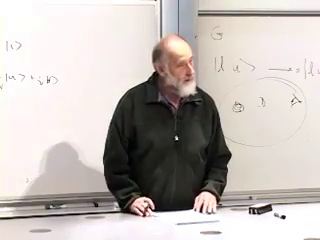
\includegraphics[width=0.66\textwidth]{lecture_07_figure_06.png}
\caption{Der begriffliche Übergang von einem festgelegten Ket zu einer Ensemblebeschreibung.}
\lectureframe{01:29:43}
\end{figure}

Wird der Zustand \(|i\rangle\) mit Wahrscheinlichkeit \(\rho_i\) präpariert, lautet der Dichteoperator
\begin{equation}
\rho=\sum_i\rho_i|i\rangle\langle i|.
\end{equation}
In der Präparationsbasis gilt
\begin{equation}
\rho=
\begin{pmatrix}
\rho_1&0&0&\cdots\\
0&\rho_2&0&\cdots\\
0&0&\rho_3&\cdots\\
\vdots&\vdots&\vdots&\ddots
\end{pmatrix}.
\end{equation}

\begin{figure}[htbp]
\centering
\includegraphics[width=0.68\textwidth]{lecture_07_figure_09.png}
\caption{Die diagonale Dichtematrix und ihre Normierungsbedingung.}
\lectureframe{01:32:12}
\end{figure}

Ihre Eigenwerte sind reell und nichtnegativ, und die Normierung der Wahrscheinlichkeiten lautet
\begin{equation}
\operatorname{Tr}\rho=\sum_i\rho_i=1.
\end{equation}

Sei \(F\) eine hermitesche Observable. Der Erwartungswert des Ensembles ist
\begin{equation}
\langle F\rangle=\operatorname{Tr}(F\rho).
\end{equation}

\begin{figure}[htbp]
\centering
\includegraphics[width=0.68\textwidth]{lecture_07_figure_10.png}
\caption{Der Erwartungswert als Spur \(\langle F\rangle=\operatorname{Tr}(F\rho)\).}
\lectureframe{01:35:05}
\end{figure}

Um den gewöhnlichen gewichteten Mittelwert zurückzugewinnen, wertet man die Spur in der Basis aus, in der \(\rho\) diagonal ist, und setzt die Vollständigkeitsrelation ein:
\begin{align}
\operatorname{Tr}(F\rho)
&=\sum_i\langle i|F\rho|i\rangle\\
&=\sum_{i,j}\langle i|F|j\rangle
               \langle j|\rho|i\rangle\\
&=\sum_i\rho_i\langle i|F|i\rangle.
\end{align}
Damit wird jeder Erwartungswert eines reinen Zustands mit der Wahrscheinlichkeit gewichtet, mit der der entsprechende Zustand präpariert wurde.

Die Spur besitzt die Zyklizitätseigenschaft
\begin{equation}
\operatorname{Tr}(AB)=\operatorname{Tr}(BA),
\end{equation}
auch wenn \(A\) und \(B\) nicht kommutieren. Daher gilt \(\operatorname{Tr}(F\rho)=\operatorname{Tr}(\rho F)\).

\section{Quantenentropie und der aufgeschobene Ertrag}

Die Entropie einer Dichtematrix ist
\begin{equation}
S(\rho)=-\operatorname{Tr}(\rho\log\rho).
\end{equation}
Für einen hermiteschen positiven Operator werden Funktionen wie \(\log\rho\) über dessen Eigenwerte definiert. Gilt
\begin{equation}
\rho=\sum_i\rho_i|i\rangle\langle i|,
\end{equation}
dann gilt
\begin{equation}
\log\rho=\sum_{\rho_i>0}(\log\rho_i)|i\rangle\langle i|,
\end{equation}
und damit
\begin{equation}
S(\rho)=-\sum_i\rho_i\log\rho_i.
\end{equation}

\begin{figure}[htbp]
\centering
\includegraphics[width=0.68\textwidth]{lecture_07_figure_11.png}
\caption{Die klassische Entropieformel, umgeschrieben als \(S=-\operatorname{Tr}(\rho\log\rho)\).}
\lectureframe{01:41:25}
\end{figure}

Ein bekannter reiner Zustand hat den Dichteoperator
\begin{equation}
\rho_\psi=|\psi\rangle\langle\psi|,
\end{equation}
mit den Eigenwerten \(1,0,\ldots\), also \(S(\rho_\psi)=0\). Das bedeutet nicht, dass jede Messung an \(|\psi\rangle\) ein sicheres Ergebnis hat. Es bedeutet, dass keine zusätzliche statistische Unkenntnis über den präparierten Zustand besteht. Am anderen Extrem gilt
\begin{equation}
\rho=\frac{I}{d}
\qquad\Longrightarrow\qquad
S(\rho)=\log d,
\end{equation}
wobei \(d=\dim\mathcal H\). Der maximal gemischte Zustand weist jeder orthogonalen Richtung das gleiche Gewicht zu.

Der Zusammenhang mit der Verschränkung ist nun nahe, aber noch nicht ausgearbeitet. Angenommen, ein zusammengesetztes System \(AB\) befindet sich in einem gemeinsamen Zustand und alle Experimente beschränken sich auf \(A\). Es muss ein Objekt geben, das jeden Erwartungswert reproduziert, der für \(A\) ermittelt werden kann, wenn \(B\) außer Acht gelassen wird. Dieses Objekt ist eine Dichtematrix für \(A\). Faktorisiert der gemeinsame Zustand, ist die Dichtematrix von \(A\) rein und hat Entropie null. Sind \(A\) und \(B\) verschränkt, ist die Dichtematrix von \(A\) im Allgemeinen gemischt und hat eine von null verschiedene Entropie. Diese reduzierte Dichtematrix zu konstruieren und ihre Entropie auszuwerten, ist die Aufgabe der nächsten Vorlesung.
